\documentclass[gr-notes.tex]{subfiles}

\begin{document}

\setcounter{chapter}{4}

\chapter{Preface to Curvature}

\setcounter{section}{7}

\section{Exercises}

\textbf{1}

(a)
Repeat the argument leading to Equation 5.1, but this time assume that only a fraction $\epsilon < 1$ of the mass's kinetic energy is converted into a photon.

If only a fraction $\epsilon$ of the energy is converted into a photon, then it will start with an energy of $\epsilon (m + mgh + \order{\boldsymbol{v}^4}$, but once it reaches the top it should have an energy of $\epsilon m$, as it loses the component due to gravitational potential energy. Thus
%
\begin{displaymath}
  \frac{E'}{E} =
  \frac{\epsilon m}{\epsilon (m + mgh + \order{\boldsymbol{v}^4)}} =
  \frac{m}{m + mgh + \order{\boldsymbol{v}^4}} =
  1 - gh + \order{\boldsymbol{v}^4}
\end{displaymath}

(b)
Assume Equation 5.1 does not hold. Devise a perpetual motion device.

If we assume that the photon does not return to an energy $m$ once it reaches the top, but instead has an energy $m' > m$, then we could create the perpetual motion device shown in Figure \ref{fig:ch5-problem-1b}. A black box consumes the photon with energy $m'$, and splits it into a new object of mass $m$, and a photon of energy $m' - m$. The object repeats the action of the original falling mass, creating an infinite loop.

\begin{figure}[h]
  \centering
  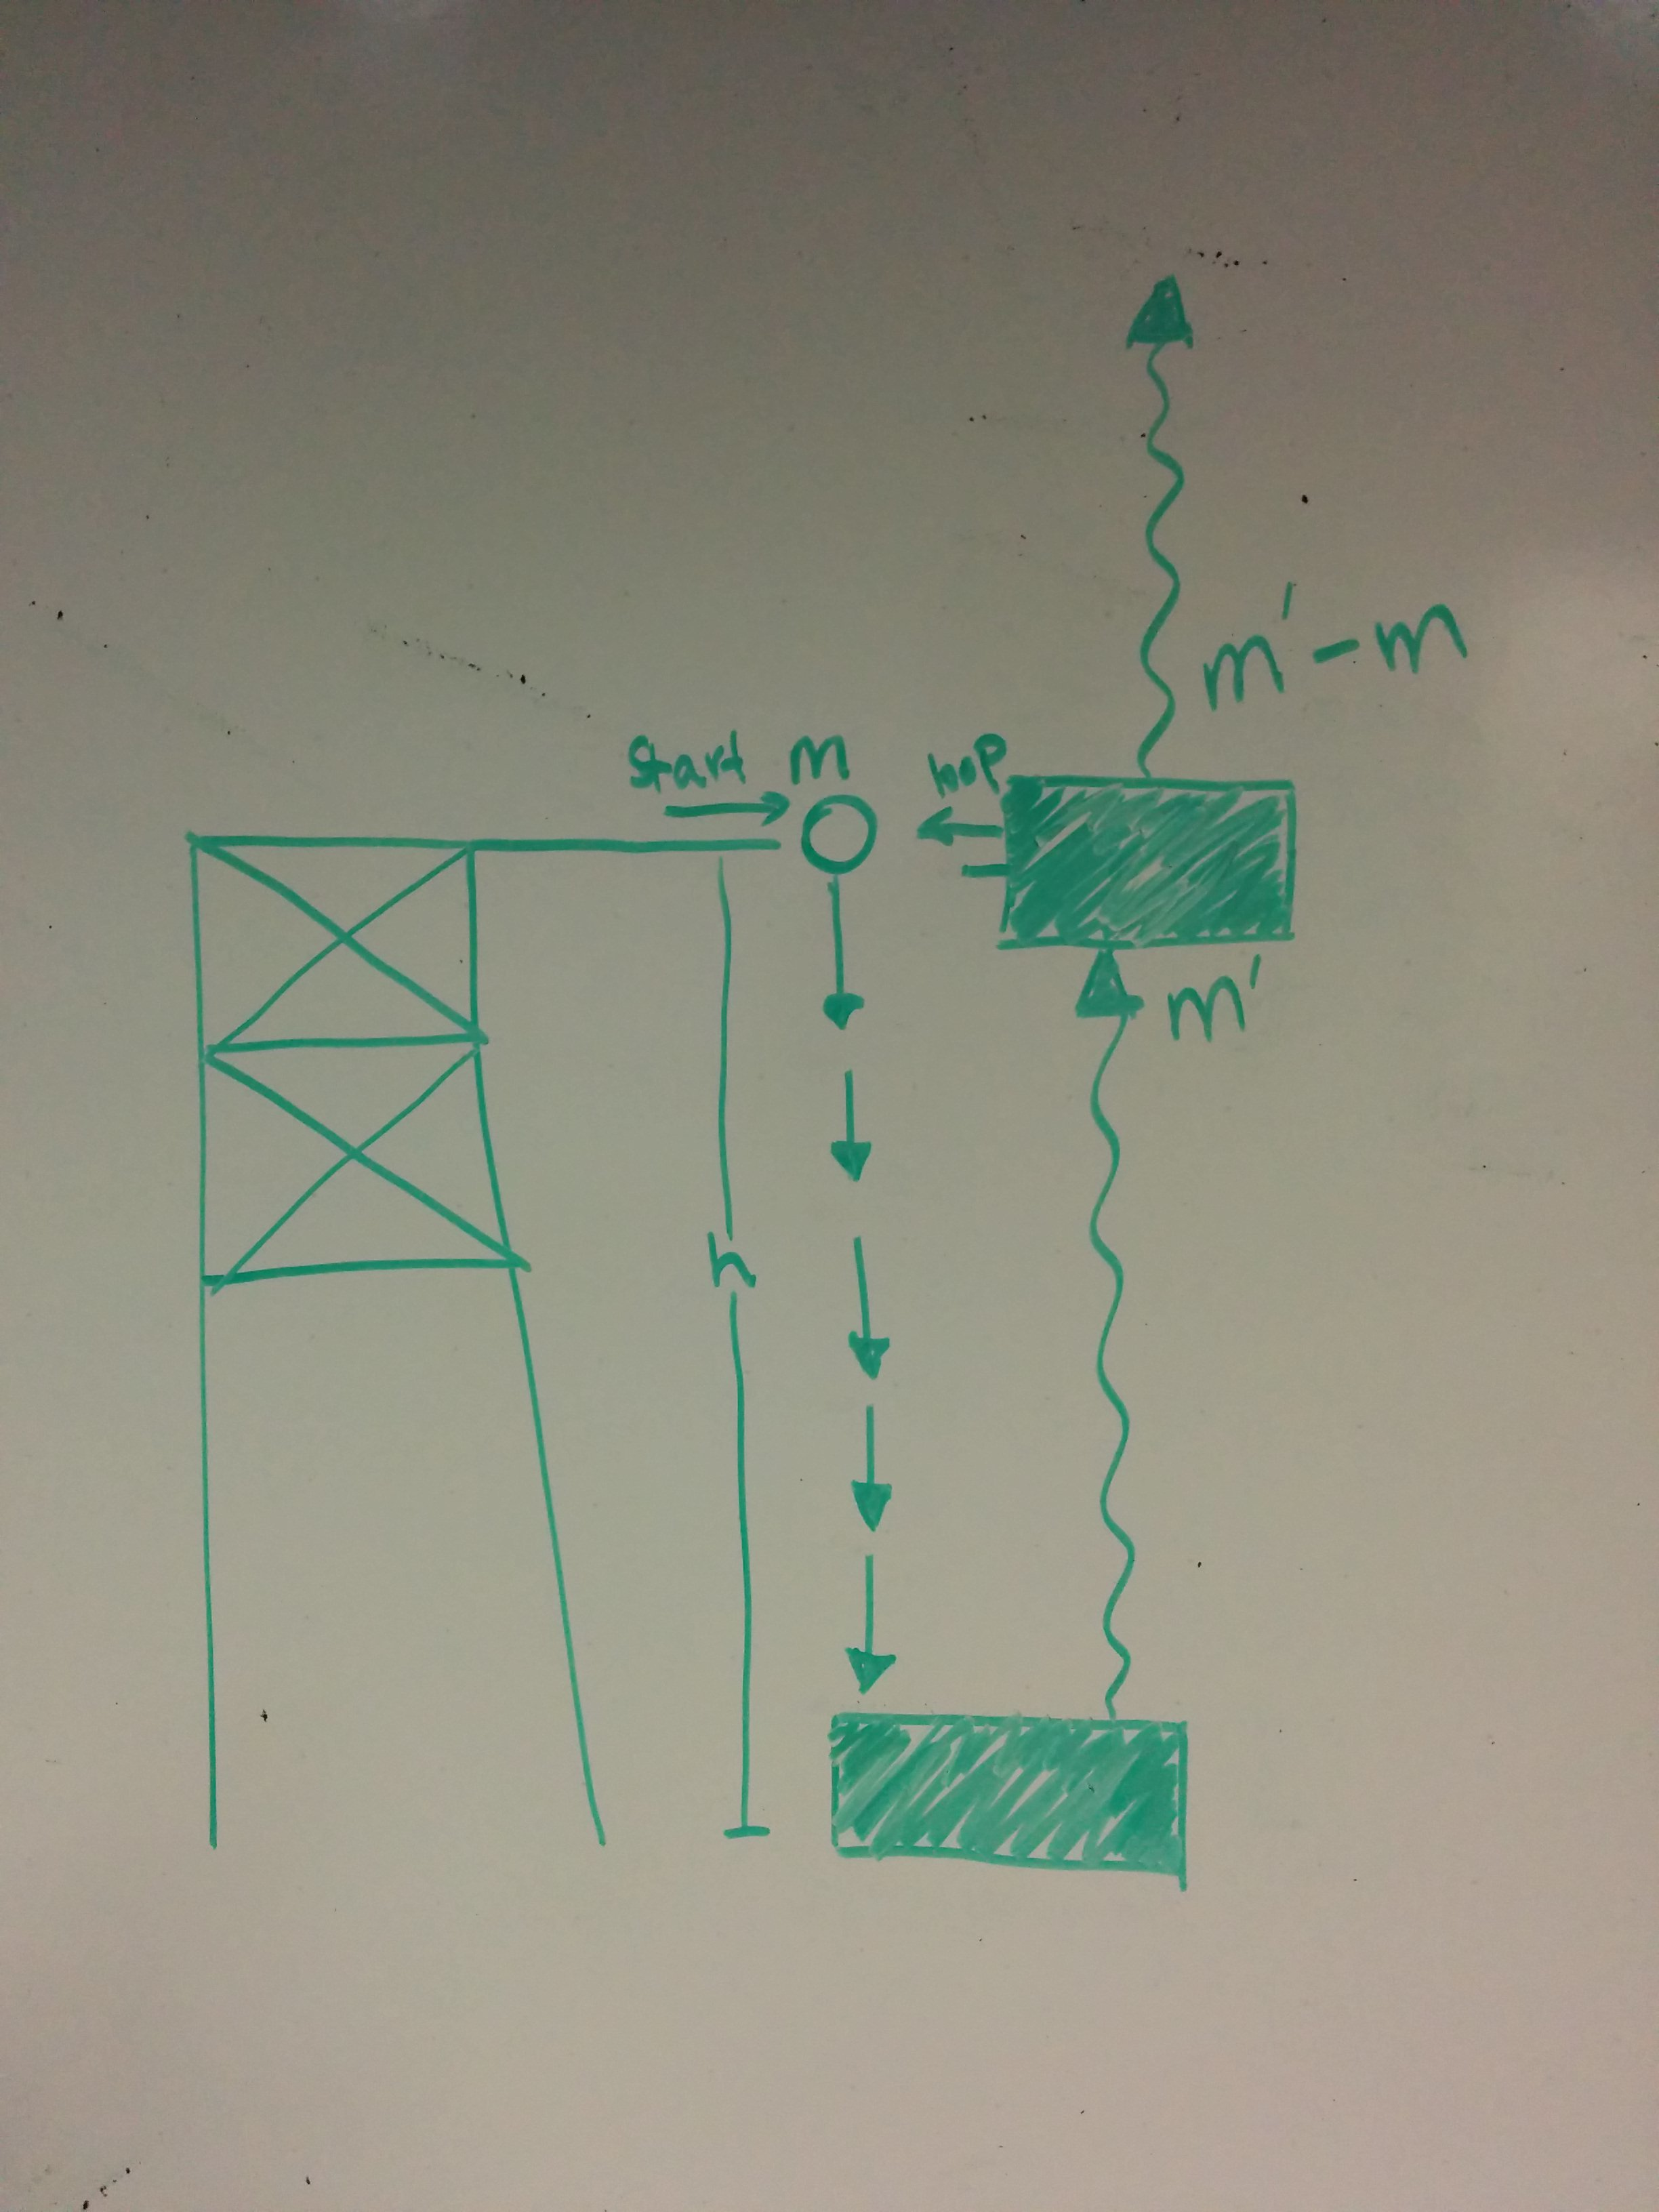
\includegraphics[width=0.75\textwidth]{img/ch5_problem_1b}
  \caption{Problem 1: Perpetual motion device.}
  \label{fig:ch5-problem-1b}
\end{figure}


\textbf{2}
Explain why a uniform gravitational field would not be able to create tides on Earth.

Tides depend on there being a gravitational field gradient. If the curvature closer to the source of the field (e.g. the Moon) is greater than it is further away, then the closer side will move towards the source more than the further side, thus creating tides. In the absense of such a gradient, there would be no difference in curvature between the two sides, and thus they would not stretch relative to each other.



\textbf{7}
Calculate the components of $\tensor{\Lambda}{^{\alpha'}_\beta}$ and $\tensor{\Lambda}{^\mu_{\nu'}}$ for transformations $(x, y) \leftrightarrow (r, \theta)$.
~
\begin{align*}
  \mqty( \Delta r \\ \Delta \theta ) &=
  \mqty( \pdv*{r}{x}      & \pdv*{r}{y} \\
         \pdv*{\theta}{x} & \pdv*{\theta}{y} )
  \mqty( \Delta x \\ \Delta y )
  &
  \mqty( \Delta x \\ \Delta y ) &=
  \mqty( \pdv*{x}{r} & \pdv*{x}{\theta} \\
         \pdv*{y}{r} & \pdv*{y}{\theta} )
  \mqty( \Delta r \\ \Delta \theta )
  \\ &=
  \mqty( x / \sqrt{x^2+y^2} & y / \sqrt{x^2 + y^2} \\
         -y / (x^2 + y^2) & x / (x^2 + y^2) )
  \mqty( \Delta x \\ \Delta y )
  &&=
  \mqty( \cos\theta & -r \sin\theta \\
         \sin\theta &  r \cos\theta )
  \mqty( \Delta r \\ \Delta \theta )
  \\ &=
  \mqty( \cos\theta & \sin\theta \\
         -(1/r) \sin\theta & (1/r) \cos\theta )
  \mqty( \Delta x \\ \Delta y )
  &&=
  \mqty( x / \sqrt{x^2 + y^2} & -y \\
         y / \sqrt{x^2 + y^2} &  x)
  \mqty( \Delta r \\ \Delta \theta )
\end{align*}
%
\begin{align*}
  \tensor{\Lambda}{^r_x} &= x / \sqrt{x^2 + y^2} = \cos\theta
  &
  \tensor{\Lambda}{^x_r} &= \cos\theta = x / \sqrt{x^2 + y^2}
  \\
  \tensor{\Lambda}{^r_y} &= y / \sqrt{x^2 + y^2} = \sin\theta
  &
  \tensor{\Lambda}{^y_r} &= \sin\theta = y / \sqrt{x^2 + y^2}
  \\
  \tensor{\Lambda}{^\theta_x} &= -y / (x^2 + y^2) = -(1/r) \sin\theta
  &
  \tensor{\Lambda}{^x_\theta} &= -r \sin\theta = -y
  \\
  \tensor{\Lambda}{^\theta_y} &= x / (x^2 + y^2) = (1/r) \cos\theta
  &
  \tensor{\Lambda}{^y_\theta} &= r \cos\theta = x
\end{align*}



\textbf{8}

(a)
$f \equiv x^2 + y^2 + 2xy$, $\vec{V} \underset{(x,y)}{\to} (x^2 + 3y, y^2 + 3x)$, $\vec{W} \underset{(r,\theta)}{\to} (1, 1)$. Express $f = f(r, \theta)$, and find the components of $\vec{V}$ and $\vec{W}$ in a polar basis, as functions of $r$ and $\theta$.

\begin{align*}
  f &= x^2 + y^2 + 2xy = (x + y)^2
  \\ &=
  (r \cos\theta + r \sin\theta)^2 =
  r^2 \sin^2\theta + r^2 \cos^2\theta + 2 r^2 \sin\theta \cos\theta
  \\ &=
  r^2 (1 + \sin(2 \theta))
  \\
%%%%%
  \vec{V} &\underset{(x,y)}{\to}
  \mqty( r^2 \cos^2\theta + 3 r \sin\theta \\
         r^2 \sin^2\theta + 3 r \cos\theta )
  \\
  \vec{V} &\underset{(r,\theta)}{\to}
  \mqty( \cos\theta & \sin\theta \\
         -(1/r) \sin\theta & (1/r) \cos\theta )
  \mqty( r^2 \cos^2\theta + 3 r \sin\theta \\
         r^2 \sin^2\theta + 3 r \cos\theta )
  \\ &\underset{(r,\theta)}{\to}
  \mqty(
    r^2 \cos^2\theta + 6 r \sin\theta \cos\theta + r^2 \sin^3\theta
    \\
    -r \cos^2\theta \sin\theta - 3 \sin^2\theta +
     r \sin^2\theta \cos\theta + 3 \cos^2\theta
  )
  \\ &\underset{(r,\theta)}{\to}
  \mqty(
    r^2 (\sin^3\theta + \cos^3\theta) + 6 r \sin\theta \cos\theta
    \\
    r \sin\theta \cos\theta (\sin\theta - \cos\theta) +
    3 (\cos^2\theta - \sin^2\theta)
  )
  \\ &\underset{(r,\theta)}{\to}
  \mqty(
    r^2 (\sin^3\theta + \cos^3\theta) + 3 r \sin(2\theta)
    \\
    (r/2) \sin(2\theta) (\sin\theta - \cos\theta) + 3 \cos(2\theta)
  )
  \\
%%%%%
  \vec{W} &\underset{(r,\theta)}{\to}
  \mqty( \cos\theta & \sin\theta \\
         -(1/r) \sin\theta & (1/r) \cos\theta )
  \mqty( 1 \\ 1 )
  \\ &\underset{(r,\theta)}{\to}
  \mqty(
    \cos\theta + \sin\theta
    \\
    (1/r) (\cos\theta - \sin\theta)
  )
\end{align*}



(b)
Express the components of $\tilde{\dd}f$ in $(x,y)$ and obtain them in $(r,\theta)$ by:

(i) using direct calculation in $(r, \theta)$:

\begin{displaymath}
  \tilde{\dd}f \underset{(r,\theta)}{\to}
  \qty( \pdv*{f}{r}, \pdv*{f}{\theta} ) =
  \qty( 2 r (1 + \sin(2 \theta)), 2 r^2 \cos(2 \theta) )
\end{displaymath}

(ii) transforming the components in $(x, y)$:

\begin{displaymath}
  \tilde{\dd}f \underset{(x,y)}{\to}
  \qty( \pdv*{f}{x}, \pdv*{f}{y} ) =
  \qty( 2 (x+y), 2 (x+y) ) =
  \qty( 2 r (\cos\theta + \sin\theta), 2 r (\cos\theta + \sin\theta))
\end{displaymath}

\begin{align*}
  \mqty( (\tilde{\dd}f)_r & (\tilde{\dd}f)_\theta ) &=
  \mqty( 1 & 1 )
  \mqty( \cos\theta & -r\sin\theta \\ \sin\theta & r\cos\theta )
  \qty[ 2 r (\cos\theta + \sin\theta) ]
  \\ &=
  \mqty( 2 r  (\cos^2\theta + \sin^2\theta + 2 \sin\theta\cos\theta) &
         2 r^2 (\cos^2\theta - \sin^2\theta) )
  \\ &=
  \mqty( 2 r (1 + \sin(2 \theta)) & 2 r^2 \cos(2 \theta) )
\end{align*}


(c)
Now find the $(r,\theta)$ components of the one-forms $\tilde{V}$ and $\tilde{W}$ associated with the vectors $\vec{V}$ and $\vec{W}$ by

(i)
using the metric tensor in $(r,\theta)$:


\begin{align*}
  V_r &=
  g_{r\alpha} V^\alpha =
  g_{rr} V^r + g_{r\theta} V^\theta
  \\ &=
  r^2 (\sin^3\theta + \cos^3\theta) + 3 r \sin(2\theta)
  \\
  V_\theta &=
  g_{\theta r} V^r + g_{\theta\theta} V^\theta =
  (1/2) r^3 \sin(2\theta) (\sin\theta - \cos\theta) +
  3 r^2 \cos(2\theta)
  \\
%%%%%
  W_r &=
  g_{r\alpha} W^\alpha =
  g_{rx} W^x + g_{ry} W^y
  \\ &=
  1 (\cos\theta + \sin\theta) +
  0 \qty[ (1/r) (\cos\theta - \sin\theta) ]
  \\ &=
  \cos\theta + \sin\theta
  \\
%%%%%
  W_\theta &=
  g_{\theta x} W^x + g_{\theta y} W^y =
  \\ &=
  0 (\cos\theta + \sin\theta) +
  r^2 \qty[ r (\cos\theta - \sin\theta) ]
  \\ &=
  r (\cos\theta - \sin\theta)
\end{align*}


(ii)
using the metric tensor in $(x,y)$ and then doing a coordinate transformation:

\begin{align*}
  V_x &= V^x; \quad V_y = V^y
  \\
  V_r &=
  \tensor{\Lambda}{^\alpha_r} V_\alpha =
  \tensor{\Lambda}{^x_r} V_x + \tensor{\Lambda}{^y_r} V_y
  \\ &=
  \cos\theta V_x + \sin\theta V_y
  \\ &=
  r^2 \cos^3\theta + (3/2) r \sin(2\theta) +
  r^2 \sin^3\theta + (3/2) r \sin(2\theta)
  \\ &=
  r^2 (\cos^3\theta + \sin^3\theta) + 3 r \sin(2\theta)
  \\
  V_\theta &=
  \tensor{\Lambda}{^\alpha_\theta} V_\alpha =
  \tensor{\Lambda}{^x_\theta} V_x + \tensor{\Lambda}{^y_\theta} V_y
  \\ &=
  (-r \sin\theta) V_x + (r \cos\theta) V_y
  \\ &=
  -r^3 \cos^2\theta \sin\theta - 3 r^2 \sin^2\theta +
   r^3 \sin^2\theta \cos\theta + 3 r^2 \cos^2\theta
  \\ &=
  r^3 \sin\theta \cos\theta (\sin\theta - \cos\theta) +
  3 r^2 (\cos^2\theta - \sin^2\theta)
  \\ &=
  (1/2) r^3 \sin(2\theta) (\sin\theta - \cos\theta) +
  3 r^2 \cos(2\theta)
  \\
%%%%%
  W_x &= W^x = W_y = W^y = 1
  \\
  W_r &=
  \tensor{\Lambda}{^\alpha_r} W_\alpha =
  \tensor{\Lambda}{^x_r} W_x + \tensor{\Lambda}{^y_r} W_y
  \\ &=
  \cos\theta + \sin\theta
  \\
  W_\theta &=
  \tensor{\Lambda}{^\alpha_\theta} W_\alpha =
  \tensor{\Lambda}{^x_\theta} W_x + \tensor{\Lambda}{^y_\theta} W_y
  \\ &=
  -r \sin\theta + r \cos\theta
  \\ &=
  r (\cos\theta - \sin\theta)
\end{align*}


\textbf{11}
Consider $V \underset{(x,y)}{\to} (x^2 + 3y, y^2 + 3x)$.

(a)
Find $\tensor{V}{^\alpha_{,\beta}}$ in Cartesian coordinates.
%
\begin{displaymath}
  \tensor{V}{^x_{,x}} = 2 x; \quad
  \tensor{V}{^y_{,y}} = 2 y; \quad
  \tensor{V}{^x_{,y}} = \tensor{V}{^y_{,x}} = 3.
\end{displaymath}

(b)
\begin{align*}
  \tensor{V}{^{\mu'}_{;\nu'}} &=
  \tensor{\Lambda}{^{\mu'}_\alpha}
  \tensor{\Lambda}{^\beta_{\nu'}}
  \tensor{V}{^\alpha_{,\beta}}
  \\
  \tensor{V}{^r_{;r}} &=
  \tensor{\Lambda}{^r_x} \tensor{\Lambda}{^x_r} \tensor{V}{^x_{,x}} +
  \tensor{\Lambda}{^r_y} \tensor{\Lambda}{^y_r} \tensor{V}{^y_{,y}} +
  \tensor{\Lambda}{^r_x} \tensor{\Lambda}{^y_r} \tensor{V}{^x_{,y}} +
  \tensor{\Lambda}{^r_y} \tensor{\Lambda}{^x_r} \tensor{V}{^y_{,x}}
  \\ &=
  (\cos^2\theta) (2r \cos\theta) +
  (\sin^2\theta) (2r \sin\theta) +
  (\sin\theta \cos\theta) (3) +
  (\sin\theta \cos\theta) (3)
  \\ &=
  2r (\cos^3\theta + \sin^3\theta) +
  3 \sin(2\theta)
  \\
  \tensor{V}{^\theta_{;\theta}} &=
  \tensor{\Lambda}{^\theta_x} \tensor{\Lambda}{^\theta_r} \tensor{V}{^x_{,x}} +
  \tensor{\Lambda}{^\theta_y} \tensor{\Lambda}{^\theta_r} \tensor{V}{^y_{,y}} +
  \tensor{\Lambda}{^\theta_x} \tensor{\Lambda}{^y_\theta} \tensor{V}{^x_{,y}} +
  \tensor{\Lambda}{^\theta_y} \tensor{\Lambda}{^\theta_r} \tensor{V}{^y_{,x}}
  \\ &=
  (\sin^2\theta) (2 r \cos\theta) + (\cos^2\theta) (2 r \sin\theta) +
  (-\sin\theta \cos\theta) (3) + (-\sin\theta \cos\theta) (3)
  \\ &=
  \sin(2\theta) [ r (\sin\theta + \cos\theta) - 3 ]
  \\
  \tensor{V}{^r_{;\theta}} &=
  \tensor{\Lambda}{^r_x} \tensor{\Lambda}{^x_\theta} \tensor{V}{^x_{,x}} +
  \tensor{\Lambda}{^r_y} \tensor{\Lambda}{^y_\theta} \tensor{V}{^y_{,y}} +
  \tensor{\Lambda}{^r_x} \tensor{\Lambda}{^y_\theta} \tensor{V}{^x_{,y}} +
  \tensor{\Lambda}{^r_y} \tensor{\Lambda}{^x_\theta} \tensor{V}{^y_{,x}}
  \\ &=
  (-r \sin\theta \cos\theta) (2 r \cos\theta) +
  (r \sin\theta \cos\theta) (2 r \sin\theta) +
  (r \cos^2\theta) (3) + (-r \sin^2\theta)
  \\ &=
  r^2 \sin(2\theta) (\sin\theta - \cos\theta) +
  3 r \cos(2 \theta)
  \\
  \tensor{V}{^\theta_{;r}} &=
  \tensor{\Lambda}{^\theta_x} \tensor{\Lambda}{^x_r} \tensor{V}{^x_{,x}} +
  \tensor{\Lambda}{^\theta_y} \tensor{\Lambda}{^y_r} \tensor{V}{^y_{,y}} +
  \tensor{\Lambda}{^\theta_x} \tensor{\Lambda}{^y_r} \tensor{V}{^x_{,y}} +
  \tensor{\Lambda}{^\theta_y} \tensor{\Lambda}{^x_r} \tensor{V}{^y_{,x}}
  \\ &=
  (-(1/r) \sin\theta \cos\theta) (2 r \cos\theta) +
  ( (1/r) \sin\theta \cos\theta) (2 r \sin\theta) +
  (-(1/r) \sin^2\theta) (3) +
  ( (1/r) \cos^2\theta) (3)
  \\ &=
  \sin(2\theta) (\sin\theta - \cos\theta) +
  \frac{3}{r} \cos(2 \theta)
\end{align*}


(c) compute $\tensor{V}{^{\mu'}_{;\nu'}}$ directly in polars using the Christoffel symbols.

Recall that we have $\tensor{\Gamma}{^\mu_{rr}} = \tensor{\Gamma}{^r_{r\theta}} = \tensor{\Gamma}{^\theta_{\theta\theta}} = 0$, $\tensor{\Gamma}{^\theta_{r\theta}} = 1/r$, and $\tensor{\Gamma}{^r_{\theta\theta}} = -r$.

\begin{align*}
  \tensor{V}{^{\mu'}_{;\nu'}} &=
  \tensor{V}{^{\mu'}_{,\nu'}} +
  \tensor{V}{^{\alpha'}} \tensor{\Gamma}{^{\mu'}_{\alpha'\nu'}}
  \\
  \tensor{V}{^r_{;r}} &=
  \tensor{V}{^r_{,r}} +
  \tensor{V}{^{\alpha'}} \tensor{\Gamma}{^r_{\alpha'r}}
  \\
  \tensor{V}{^r_{,r}} &=
  \pdv*{V^r}{r} =
  2 r (\sin^3\theta + \cos^3\theta) + 3 \sin(2\theta)
  \\
  \tensor{V}{^\alpha} \tensor{\Gamma}{^r_{\alpha r}} &=
  V^r     \tensor{\Gamma}{^r_{rr}} +
  V^\theta \tensor{\Gamma}{^r_{\theta r}} =
  0
  \\
  \tensor{V}{^r_{;r}} &=
  \tensor{V}{^r_{,r}} =
  2 r (\sin^3\theta + \cos^3\theta) + 3 \sin(2\theta)
  \\
  \tensor{V}{^\theta_{;\theta}} &=
  \tensor{V}{^\theta_{,\theta}} +
  \tensor{V}{^{\alpha'}} \tensor{\Gamma}{^\theta_{\alpha'\theta}}
  \\
  \tensor{V}{^\theta_{,\theta}} &=
  \pdv*{V^\theta}{\theta} =
  (r/2) \sin(2\theta) (\sin\theta + \cos\theta) +
  r \cos(2\theta) (\sin\theta - \cos\theta) -
  6 \sin(2\theta)
  \\
  \tensor{V}{^{\alpha'}} \tensor{\Gamma}{^\theta_{\alpha'\theta}} &=
  \tensor{V}{^r} \tensor{\Gamma}{^\theta_{r\theta}} +
  \tensor{V}{^\theta} \tensor{\Gamma}{^\theta_{\theta\theta}}
  \\ &=
  [r^2 (\sin^3\theta + \cos^3\theta) + 3r \sin(2\theta)] (1/r)
  \\ &=
  r (\sin^3\theta + \cos^3\theta) + 3 \sin(2\theta)
  \\
  \tensor{V}{^\theta_{;\theta}} &=
  \sin(2\theta) [r (\sin\theta + \cos\theta) - 3]
  \\
  \tensor{V}{^r_{;\theta}} &=
  \tensor{V}{^r_{,\theta}} +
  V^r \tensor{\Gamma}{^r_{r\theta}} +
  V^\theta \tensor{\Gamma}{^r_{\theta\theta}}
  \\ &=
  \tensor{V}{^r_{,\theta}} +
  V^\theta \tensor{\Gamma}{^r_{\theta\theta}} =
  \pdv*{V^r}{\theta} - r V^\theta
  \\ &=
  6 r \cos(2\theta) +
  (3/2) r^2 \sin(2\theta) (\sin\theta-\cos\theta) -
  ((1/2) r^2 \sin(2\theta) (\sin\theta - \cos\theta) + 3 r \cos(2\theta))
  \\ &=
  r^2 \sin(2\theta) (\sin\theta - \cos\theta) + 3 r \cos(2\theta)
  \\
  \tensor{V}{^\theta_{;r}} &=
  \tensor{V}{^\theta_{,r}} +
  V^r \tensor{\Gamma}{^\theta_{rr}} +
  V^\theta \tensor{\Gamma}{^\theta_{\theta r}} =
  \tensor{V}{^\theta_{,r}} +
  \frac{1}{r}
  V^\theta
  \\ &=
  (1/2) \sin(2\theta) (\sin\theta - \cos\theta) +
  (1/2) \sin(2\theta) (\sin\theta - \cos\theta) +
  (3/r) \cos(2\theta)
  \\ &=
  \sin(2\theta) (\sin\theta - \cos\theta) +
  (3/r) \cos(2\theta)
\end{align*}


(d)
Calculate the divergence using the results from part (a)
%
\begin{displaymath}
  \tensor{V}{^\alpha_{,\alpha}} =
  \tensor{V}{^x_{,x}} + \tensor{V}{^y_{,y}} =
  2 (x + y) =
  2 r (\sin\theta + \cos\theta)
\end{displaymath}


(e)
Calculate the divergence using the results from either part (b) or (c).
%
\begin{align*}
  \tensor{V}{^{\mu'}_{;\mu'}} &=
  \tensor{V}{^{r}_{;r}} +
  \tensor{V}{^{\theta}_{;\theta}}
  \\ &=
  2 r (\sin^3\theta + \cos^3\theta) +
  3 \sin(2\theta) +
  \sin(2\theta) [r (\sin\theta + \cos\theta) - 3]
  \\ &=
  2 r (\sin\theta + \cos\theta)
\end{align*}



(f)
Compute $\tensor{V}{^{\mu'}_{;\mu'}}$ using Equation 5.56.

\begin{displaymath}
  \tensor{V}{^{\mu'}_{;\mu'}} =
  \frac{1}{r} \pdv{r} (r V^r) + \pdv{\theta} (V^\theta) =
  2 r (\sin\theta + \cos\theta)
\end{displaymath}




\textbf{12}
%
\begin{displaymath}
  \tilde{p} \underset{(x,y)}{\to} (x^2 + 3y, y^2 + 3x).
\end{displaymath}

(a)
Find the components $p_{\alpha,\beta}$ in Cartesian coordinates.

Since $p_{\alpha,\beta} = \pdv*{p_\alpha}{x^\beta}$, it's simply $p_{x,x} = 2x$, $p_{y,y} = 2y$, and $p_{x,y} = p_{y,x} = 3$.

(b)
Find the components $p_{\mu';\nu'}$ in polar coordinates by using the transformation $\tensor{\Lambda}{^\alpha_{\mu'}} \tensor{\Lambda}{^\beta_{\nu'}} p_{\alpha,\beta}$.

\begin{align*}
  p_{r;r} &=
  \qty(\tensor{\Lambda}{^x_r})^2 p_{x,x} +
  \qty(\tensor{\Lambda}{^y_r})^2 p_{y,y} +
  2 \tensor{\Lambda}{^x_r} \tensor{\Lambda}{^y_r} p_{x,y}
  \\ &=
  (\cos^2\theta) (2 r \cos\theta) +
  (\sin^2\theta) (2 r \sin\theta) +
  2 (\sin\theta \cos\theta) (3)
  \\ &=
  2 r (\sin^3\theta + \cos^3\theta) + 3 \sin(2\theta)
  \\
  p_{\theta;\theta} &=
  \qty(\tensor{\Lambda}{^x_\theta})^2 p_{x,x} +
  \qty(\tensor{\Lambda}{^y_\theta})^2 p_{y,y} +
  2 \tensor{\Lambda}{^x_\theta} \tensor{\Lambda}{^y_\theta} p_{x,y}
  \\ &=
  (-r \sin\theta)^2 (2 r \cos\theta) +
  (r \cos\theta)^2 (2 r \sin\theta) +
  2 (3 (-r \sin\theta) (r \cos\theta))
  \\ &=
  r^2 \sin(2\theta) (r (\sin\theta + \cos\theta) - 3)
  \\
  p_{r;\theta} &=
  \tensor{\Lambda}{^x_r} \tensor{\Lambda}{^x_\theta} p_{x,x} +
  \tensor{\Lambda}{^y_r} \tensor{\Lambda}{^y_\theta} p_{y,y} +
  \tensor{\Lambda}{^x_r} \tensor{\Lambda}{^y_\theta} p_{x,y} +
  \tensor{\Lambda}{^y_r} \tensor{\Lambda}{^x_\theta} p_{y,x}
  \\ &=
  (-r \sin\theta \cos\theta) (2 r \cos\theta) +
  (r \sin\theta \cos\theta) (2 r \sin\theta) +
  3 (r \cos^2\theta - r \sin^2\theta)
  \\ &=
  r^2 \sin(2\theta) (\sin\theta - \cos\theta) + 3 r \cos(2\theta),
\end{align*}
and by the symmetry of $p_{\alpha,\beta}$ in Cartesian coordinates, $p_{\theta;r} = p_{r;\theta}$.

(c)
Now find $p_{\mu';\nu'}$ using the Christoffel symbols.

\begin{align*}
  p_{r;r} &=
  p_{r,r} -
  p_r \tensor{\Gamma}{^r_{rr}} -
  p_\theta \tensor{\Gamma}{^\theta_{rr}} =
  p_{r,r} = \pdv*{p_r}{r}
  \\ &=
  \pdv*{r} \qty[ r^2 (\cos^3\theta + \sin^3\theta) + 3 r \sin(2\theta) ] =
  2 r (sin^3\theta + \cos^3\theta) + 3 \sin(2\theta)
  \\
  p_{\theta;\theta} &=
  p_{\theta,\theta} -
  p_r \tensor{\Gamma}{^r_{\theta\theta}} -
  p_\theta \tensor{\Gamma}{^\theta_{\theta\theta}} =
  p_{\theta,\theta} + r p_r =
  \pdv*{p_\theta}{\theta}
  \\ &=
  \pdv*{\theta} \qty[
    (1/2) r^3 \sin(2\theta) (\sin\theta - \cos\theta) +
    3 r^2 \cos(2\theta)
  ] +
  r \qty[
    r^2 (\cos^3\theta + \sin^3\theta) + 3 r \sin(2\theta)
  ]
  \\ &=
  r^2 \sin(2\theta) \qty[ r (\sin\theta + \cos\theta) - 3 ]
  \\
  p_{r;\theta} &=
  p_{r,\theta} -
  p_r \tensor{\Gamma}{^r_{r\theta}} -
  p_\theta \tensor{\Gamma}{^\theta_{r\theta}} =
  \pdv*{p_r}{\theta} - (1/r) p_\theta
  \\ &=
  r^2 \sin(2\theta) (\sin\theta - \cos\theta) + 3 r \cos(2\theta)
  \\
  p_{\theta;r} &=
  p_{\theta,r} -
  p_r \tensor{\Gamma}{^r_{\theta r}} -
  p_\theta \tensor{\Gamma}{^\theta_{\theta r}} =
  \pdv*{p_\theta}{r} - (1/r) p_\theta
  \\ &=
  r^2 \sin(2\theta) (\sin\theta - \cos\theta) + 3 r \cos(2\theta)
\end{align*}


\textbf{13}
Show in polars that $g_{\mu'\nu'} \tensor{V}{^{\alpha'}_{;\nu'}} = p_{\mu';\nu'}$.

\begin{align*}
  g_{r\alpha'} \tensor{V}{^{\alpha'}_{;r}} &=
  g_{rr} \tensor{V}{^{r}_{;r}} + g_{r\theta} \tensor{V}{^{\theta}_{;r}}
  \\ &=
  1 \tensor{V}{^r_{;r}} =
  p_{r;r}
  \\
  g_{\theta\alpha'} \tensor{V}{^{\alpha'}_{;\theta}} &=
  g_{\theta r} \tensor{V}{^r_{;\theta}} +
  g_{\theta\theta} \tensor{V}{^\theta_{;\theta}}
  \\ &=
  r^2 \tensor{V}{^\theta_{;\theta}} =
  p_{\theta;\theta}
  \\
  g_{r \alpha'} \tensor{V}{^{\alpha'}_{;\theta}} &=
  g_{rr} \tensor{V}{^r_{;\theta}} +
  g_{r\theta} \tensor{V}{^\theta_{;\theta}}
  \\ &=
  1 \tensor{V}{^r_{;\theta}} =
  p_{\theta;r}
  \\
  g_{\theta\alpha'} \tensor{V}{^{\alpha'}_{;r}} &=
  g_{\theta r} \tensor{V}{^r_{;r}} +
  g_{\theta\theta} \tensor{V}{^\theta_{;r}}
  \\ &=
  r^2 \tensor{V}{^\theta_{;r}} =
  p_{\theta;r}
\end{align*}


\textbf{14}
Compute $\grad_\beta A^{\mu\nu}$ for the tensor $\boldsymbol{A}$ with components:
%
\begin{align*}
  A^{rr} &= r^2, & A^{r\theta} &= r \sin\theta,
  \\
  A^{\theta\theta} &= \tan\theta, & A^{\theta r} &= r \cos\theta
\end{align*}
%
\begin{align*}
  \tensor{A}{^{rr}_{,r}} &= 2r &
  \tensor{A}{^{rr}_{,\theta}} &= 0
  \\
  \tensor{A}{^{\theta\theta}_{,r}} &= 0 &
  \tensor{A}{^{\theta\theta}_{,\theta}} &= \sec^2\theta
  \\
  \tensor{A}{^{r\theta}_{,r}} &= \sin\theta &
  \tensor{A}{^{r\theta}_{,\theta}} &= r \cos\theta
  \\
  \tensor{A}{^{\theta r}_{,r}} &= \cos\theta &
  \tensor{A}{^{\theta r}_{,\theta}} &= -r \sin\theta
\end{align*}
%
\begin{displaymath}
  \grad_\beta A^{\mu \nu} =
  \tensor{A}{^{\mu \nu}_{,\beta}} +
  A^{\alpha \nu} \tensor{\Gamma}{^\mu_{\alpha \beta}} +
  A^{\mu \alpha} \tensor{\Gamma}{^\nu_{\alpha \beta}}
\end{displaymath}
%
\begin{align*}
  \grad_r A^{rr} &=
  \tensor{A}{^{rr}_{,r}} +
  A^{\alpha r} \tensor{\Gamma}{^r_{\alpha r}} +
  A^{r\alpha} \tensor{\Gamma}{^r_{\alpha r}}
  \\ &=
  \tensor{A}{^{rr}_{,r}} +
  A^{r r} \tensor{\Gamma}{^r_{r r}} +
  A^{\theta r} \tensor{\Gamma}{^r_{\theta r}} +
  A^{r r} \tensor{\Gamma}{^r_{r r}} +
  A^{r \theta} \tensor{\Gamma}{^r_{\theta r}}
  \\ &=
  \tensor{A}{^{rr}_{,r}} =
  2 r
  \\
  \grad_\theta A^{r r} &=
  \tensor{A}{^{r r}_{,\theta}} +
  A^{\alpha r} \tensor{\Gamma}{^r_{\alpha \theta}} +
  A^{r \alpha} \tensor{\Gamma}{^r_{\alpha \theta}}
  \\ &=
  \tensor{A}{^{r r}_{,\theta}} +
  A^{r r} \tensor{\Gamma}{^r_{r \theta}} +
  A^{\theta r} \tensor{\Gamma}{^r_{\theta \theta}} +
  A^{r r} \tensor{\Gamma}{^r_{r \theta}} +
  A^{r \theta} \tensor{\Gamma}{^r_{\theta \theta}}
  \\ &=
  (A^{\theta r} + A^{r \theta}) \tensor{\Gamma}{^r_{\theta \theta}} =
  -r^2 (\sin\theta + \cos\theta)
  \\
  \grad_r A^{\theta \theta} &=
  \tensor{A}{^{\theta \theta}_{,r}} +
  A^{\alpha \theta} \tensor{\Gamma}{^\theta_{\alpha r}} +
  A^{\theta \alpha} \tensor{\Gamma}{^\theta_{\alpha r}}
  \\ &=
  \tensor{A}{^{\theta \theta}_{,r}} +
  A^{r \theta} \tensor{\Gamma}{^\theta_{r r}} +
  A^{\theta \theta} \tensor{\Gamma}{^\theta_{\theta r}} +
  A^{\theta r} \tensor{\Gamma}{^\theta_{r r}} +
  A^{\theta \theta} \tensor{\Gamma}{^\theta_{\theta r}}
  \\ &=
  2 A^{\theta \theta} \tensor{\Gamma}{^\theta_{\theta r}} =
  (2/r) \tan\theta
  \\
  \grad_\theta A^{\theta \theta} &=
  \tensor{A}{^{\theta \theta}_{,\theta}} +
  A^{\alpha \theta} \tensor{\Gamma}{^\theta_{\alpha \theta}} +
  A^{\theta \alpha} \tensor{\Gamma}{^\theta_{\alpha \theta}}
  \\ &=
  \tensor{A}{^{\theta \theta}_{,\theta}} +
  A^{r \theta} \tensor{\Gamma}{^\theta_{r \theta}} +
  A^{\theta \theta} \tensor{\Gamma}{^\theta_{\theta \theta}} +
  A^{\theta r} \tensor{\Gamma}{^\theta_{r \theta}} +
  A^{\theta \theta} \tensor{\Gamma}{^\theta_{\theta \theta}}
  \\ &=
  \tensor{A}{^{\theta \theta}_{,\theta}} +
  (A^{r \theta} + A^{\theta r}) \tensor{\Gamma}{^\theta_{r \theta}} =
  \sin\theta + \cos\theta + \sec^2\theta
  \\
  \grad_r A^{r \theta} &=
  \tensor{A}{^{r \theta}_{,r}} +
  A^{\alpha \theta} \tensor{\Gamma}{^r_{\alpha r}} +
  A^{r \alpha} \tensor{\Gamma}{^\theta_{\alpha r}}
  \\ &=
  \tensor{A}{^{r \theta}_{,r}} +
  A^{r \theta} \tensor{\Gamma}{^r_{r r}} +
  A^{\theta \theta} \tensor{\Gamma}{^r_{\theta r}} +
  A^{r r} \tensor{\Gamma}{^\theta_{r r}} +
  A^{r \theta} \tensor{\Gamma}{^\theta_{\theta r}}
  \\ &=
  \tensor{A}{^{r \theta}_{,r}} +
  A^{r \theta} \tensor{\Gamma}{^\theta_{\theta r}} =
  2 \sin\theta
  \\
  \grad_\theta A^{r \theta} &=
  \tensor{A}{^{r \theta}_{,\theta}} +
  A^{\alpha \theta} \tensor{\Gamma}{^r_{\alpha \theta}} +
  A^{r \alpha} \tensor{\Gamma}{^\theta_{\alpha \theta}}
  \\ &=
  \tensor{A}{^{r \theta}_{,\theta}} +
  A^{r \theta} \tensor{\Gamma}{^r_{r \theta}} +
  A^{\theta \theta} \tensor{\Gamma}{^r_{\theta \theta}} +
  A^{r r} \tensor{\Gamma}{^\theta_{r \theta}} +
  A^{r \theta} \tensor{\Gamma}{^\theta_{\theta \theta}}
  \\ &=
  \tensor{A}{^{r \theta}_{,\theta}} +
  A^{\theta \theta} \tensor{\Gamma}{^r_{\theta \theta}} +
  A^{r r} \tensor{\Gamma}{^\theta_{r \theta}} =
  r (1 + \cos\theta - \tan\theta)
  \\
  \grad_r A^{\theta r} &=
  \tensor{A}{^{\theta r}_{,r}} +
  A^{\alpha r} \tensor{\Gamma}{^\theta_{\alpha r}} +
  A^{\theta \alpha} \tensor{\Gamma}{^r_{\alpha r}}
  \\ &=
  \tensor{A}{^{\theta r}_{,r}} +
  A^{r r} \tensor{\Gamma}{^\theta_{r r}} +
  A^{\theta r} \tensor{\Gamma}{^\theta_{\theta r}} +
  A^{\theta r} \tensor{\Gamma}{^r_{r r}} +
  A^{\theta \theta} \tensor{\Gamma}{^r_{\theta r}}
  \\ &=
  \tensor{A}{^{\theta r}_{,r}} +
  A^{\theta r} \tensor{\Gamma}{^\theta_{\theta r}} =
  2 \cos\theta
  \\
  \grad_\theta A^{\theta r} &=
  \tensor{A}{^{\theta r}_{,\theta}} +
  A^{\alpha r} \tensor{\Gamma}{^\theta_{\alpha \theta}} +
  A^{\theta \alpha} \tensor{\Gamma}{^r_{\alpha \theta}}
  \\ &=
  \tensor{A}{^{\theta r}_{,\theta}} +
  A^{r r} \tensor{\Gamma}{^\theta_{r \theta}} +
  A^{\theta r} \tensor{\Gamma}{^\theta_{\theta \theta}} +
  A^{\theta r} \tensor{\Gamma}{^r_{r \theta}} +
  A^{\theta \theta} \tensor{\Gamma}{^r_{\theta \theta}}
  \\ &=
  \tensor{A}{^{\theta r}_{,\theta}} +
  A^{r r} \tensor{\Gamma}{^\theta_{r \theta}} +
  A^{\theta \theta} \tensor{\Gamma}{^r_{\theta \theta}} =
  -r \sin\theta
\end{align*}


\textbf{15}
Find the components of $\tensor{V}{^\alpha_{;\beta;\gamma}}$ for the vector $V^r = 1$, $V^\theta = 0$.

We start by finding the components of $\tensor{V}{^\alpha_{;\beta}}$.
%
\begin{displaymath}
  \tensor{V}{^\alpha_{;\beta}} =
  \tensor{V}{^\alpha_{,\beta}} +
  V^\mu \tensor{\Gamma}{^\alpha_{\mu\beta}}.
\end{displaymath}
%
By noting that $\tensor{V}{^\alpha_{,\beta}} = V^\theta = \tensor{\Gamma}{^r_{rr}} = \tensor{\Gamma}{^r_{r\theta}} = 0$, we can simplify this to
%
\begin{displaymath}
  \tensor{V}{^\alpha_{;\beta}} =
  V^r \tensor{\Gamma}{^\alpha_{r\beta}},
\end{displaymath}
%
which means
%
\begin{displaymath}
  \tensor{V}{^r_{;r}} = \tensor{V}{^r_{;\theta}} = \tensor{V}{^\theta_{;r}} = 0;
  \quad
  \tensor{V}{^\theta_{;\theta}} = \frac{1}{r}.
\end{displaymath}
%
Now we can say
%
\begin{displaymath}
  \tensor{V}{^\alpha_{;\beta;\mu}} =
  \grad_\mu \tensor{V}{^\alpha_{;\beta}} =
  \tensor{V}{^\alpha_{;\beta,\mu}} +
  \tensor{V}{^\gamma_{;\beta}} \tensor{\Gamma}{^\alpha_{\gamma\mu}} -
  \tensor{V}{^\alpha_{;\gamma}} \tensor{\Gamma}{^\gamma_{\beta\mu}}.
\end{displaymath}
%
Note that $\tensor{V}{^\theta_{;\theta}}$ is a function only of $r$, and so $\tensor{V}{^\theta_{;\theta,r}} = -1/r^2$, and all other partial derivatives are zero. We can also see by inspecting the components, that $\tensor{V}{^r_{;\mu;\nu}} = \tensor{V}{^\theta_{;\mu}} \tensor{\Gamma}{^r_{\theta\mu}}$, as all other components go to zero. Likewise, we can see that $\tensor{V}{^\theta_{;r;\mu}} = -\tensor{V}{^\theta_{;\theta}} \tensor{\Gamma}{^\theta_{r\mu}}$. It then becomes easy to find all the individual components. I summarize their values in Table \ref{tab:ch5-ex15}.

\begin{table}[b]
  \centering
  \begin{tabular}{ccc|c}
    $\alpha$ &  $\beta$ &    $\mu$ & $\tensor{V}{^\alpha_{;\beta;\mu}}$ \\
    \hline
    $\theta$ & $\theta$ & $\theta$ & $0$      \\
    $\theta$ & $\theta$ &      $r$ & $-1/r^2$ \\
    $\theta$ &      $r$ & $\theta$ & $-1/r^2$ \\
    $\theta$ &      $r$ &      $r$ & $0$      \\
         $r$ & $\theta$ & $\theta$ & $-1$     \\
         $r$ & $\theta$ &      $r$ & $0$      \\
         $r$ &      $r$ & $\theta$ & $0$      \\
         $r$ &      $r$ &      $r$ & $0$      \\
  \end{tabular}
  \caption{Components of the tensor in Exercise 15.}
  \label{tab:ch5-ex15}
\end{table}


\textbf{16}
Repeat the steps leading from Equation 5.74 to 5.75.

Recalling that $g_{\alpha\mu;\beta} = 0$, we can rewrite Equation 5.72 as
%
\begin{displaymath}
  g_{\alpha\beta,\mu} =
  \tensor{\Gamma}{^\nu_{\alpha\mu}} g_{\nu\beta} +
  \tensor{\Gamma}{^\nu_{\beta\mu}} g_{\alpha\nu}.
\end{displaymath}
%
Now if we switch the $\beta$ and $\mu$ indices, and then switch the $\alpha$ and $\beta$ indices, we get two more equations,
%
\begin{align*}
  g_{\alpha\mu,\beta} &=
  \tensor{\Gamma}{^\nu_{\alpha\beta}} g_{\nu\mu} +
  \tensor{\Gamma}{^\nu_{\mu\beta}} g_{\alpha\nu},
  \\*
  g_{\beta\mu,\alpha} &=
  \tensor{\Gamma}{^\nu_{\beta\alpha}} g_{\nu\mu} +
  \tensor{\Gamma}{^\nu_{\mu\alpha}} g_{\beta\nu}.
\end{align*}
%
Now we add the first two equations and subtract the third, getting
%
\begin{align*}
  g_{\alpha\beta,\mu} + g_{\alpha\mu,\beta} - g_{\beta\mu,\alpha} &=
  \tensor{\Gamma}{^\nu_{\alpha\mu}} g_{\nu\beta} +
  \tensor{\Gamma}{^\nu_{\beta\mu}} g_{\alpha\nu} +
  \tensor{\Gamma}{^\nu_{\alpha\beta}} g_{\nu\mu} +
  \tensor{\Gamma}{^\nu_{\mu\beta}} g_{\alpha\nu} -
  \tensor{\Gamma}{^\nu_{\beta\alpha}} g_{\nu\mu} -
  \tensor{\Gamma}{^\nu_{\mu\alpha}} g_{\beta\nu}
  \\ &=
  {\color{red}
  \tensor{\Gamma}{^\nu_{\alpha\mu}} g_{\beta\nu}} +
  {\color{green}
  \tensor{\Gamma}{^\nu_{\beta\mu}} g_{\alpha\nu}} +
  {\color{blue}
  \tensor{\Gamma}{^\nu_{\alpha\beta}} g_{\nu\mu}} +
  {\color{green}
  \tensor{\Gamma}{^\nu_{\beta\mu}} g_{\alpha\nu}} -
  {\color{red}
  \tensor{\Gamma}{^\nu_{\alpha\beta}} g_{\nu\mu}} -
  {\color{blue}
  \tensor{\Gamma}{^\nu_{\alpha\mu}} g_{\beta\nu}}
  \\ &=
  2 \tensor{\Gamma}{^\nu_{\beta\mu}} g_{\alpha\nu}.
\end{align*}
%
Recalling that $g^{\alpha\gamma} g_{\alpha\nu} = \tensor{g}{^\gamma_\nu} = \tensor{\delta}{^\gamma_\nu}$, we divide both sides by $2$ and multiply by $g^{\alpha\gamma}$, arriving at Equation 5.75:
%
\begin{align*}
  \frac{1}{2}
  g^{\alpha\gamma}
  (g_{\alpha\beta,\mu} + g_{\alpha\mu,\beta} - g_{\beta\mu,\alpha} &=
  \frac{2}{2}
  g^{\alpha\gamma} g_{\alpha\nu}
  \tensor{\Gamma}{^\nu_{\beta\mu}}
  \\ &=
  \tensor{\Gamma}{^\nu_{\beta\mu}}
\end{align*}


\textbf{17}
Show how $\tensor{V}{^\beta_{,\alpha}}$ and $V^\mu \tensor{\Gamma}{^\beta_{\upsilon\alpha}}$ transform under change of coordinates. Neither follows a tensor transformation law, but their \emph{sum} does.

\begin{align*}
  \tensor{V}{^{\alpha'}_{,\beta'}} &=
  \pdv{V^{\alpha'}}{x^{\beta'}} =
  \tensor{\Lambda}{^\beta_{\beta'}}
  \pdv{x^\beta} \qty[ \tensor{\Lambda}{^{\alpha'}_\alpha} V^\alpha ]
  \\ &=
  \tensor{\Gamma}{^\beta_{\beta'}} \qty[
    V^\alpha \pdv{x^\beta} \tensor{\Lambda}{^{\alpha'}_\alpha} +
    \tensor{\Lambda}{^{\alpha'}_\alpha} \pdv{x^\beta} V^\alpha
  ]
  \\ &=
  \tensor{\Lambda}{^\beta_{\beta'}} V^\alpha
  \tensor{\Lambda}{^{\alpha'}_{\alpha,\beta}} +
  \tensor{\Lambda}{^\beta_{\beta'}} \tensor{\Lambda}{^{\alpha'}_\alpha}
  \tensor{V}{^\alpha_{,\beta}}
  \\ &\neq
  \tensor{\Lambda}{^\beta_{\beta'}} \tensor{\Lambda}{^{\alpha'}_\alpha}
  \tensor{V}{^\alpha_{,\beta}}
  \\
  \pdv{\vec{e}_{\alpha'}}{x^{\beta'}} &=
  \tensor{\Lambda}{^\beta_{\beta'}}
  \pdv{x^\beta} \qty[ \tensor{\Lambda}{^\alpha_{\alpha'}} \vec{e}_\alpha ]
  \\ &=
  \tensor{\Lambda}{^\beta_{\beta'}} \qty[
    \tensor{\Lambda}{^\alpha_{\alpha'}} \pdv{x^\beta} \vec{e}_\alpha +
    \vec{e}_\alpha \pdv{x^\beta} \tensor{\Lambda}{^\alpha_{\alpha'}}
  ]
  \\ &=
  \tensor{\Lambda}{^\beta_{\beta'}}
  \tensor{\Lambda}{^\alpha_{\alpha'}}
  \tensor{\Gamma}{^\mu_{\alpha\beta}} \vec{e}_\mu +
  \tensor{\Lambda}{^\beta_{\beta'}}
  \tensor{\Lambda}{^\alpha_{\alpha',\beta}}
  \vec{e_\alpha}
  \\ &\neq
  \tensor{\Lambda}{^\beta_{\beta'}}
  \tensor{\Lambda}{^\alpha_{\alpha'}}
  \tensor{\Gamma}{^\mu_{\alpha\beta}} \vec{e}_\mu,
\end{align*}
%
so we have shown that $\pdv*{\vec{e}_{\alpha'}}{x^{\beta'}}$ is not a tensor,
and since $\tensor{V}{^\mu}$ is a tensor, and the product of a tensor and a non-tensor is also not a tensor, then $V^\mu\tensor{\Gamma}{^\beta_{\nu\alpha}}$ is not a tensor.

According to Carroll, the precise transformation is
%
\begin{displaymath}
  \tensor{\Gamma}{^{\nu'}_{\mu'\lambda'}} =
  \tensor{\Lambda}{^\mu_{\mu'}}
  \tensor{\Lambda}{^\lambda_{\lambda'}}
  \tensor{\Lambda}{^{\nu'}_\nu}
  \tensor{\Gamma}{^\nu_{\mu\lambda}} +
  \tensor{\Lambda}{^\mu_{\mu'}}
  \tensor{\Lambda}{^\lambda_{\lambda'}}
  \tensor{\Lambda}{^{\nu'}_{\mu\lambda}}.
\end{displaymath}
%
Now we add the two expressions, in order to show that it is a tensor equation
%
\begin{align*}
  \tensor{V}{^{\nu'}_{,\lambda'}} +
  V^{\mu'} \tensor{\Gamma}{^{\nu'}_{\mu'\lambda'}} &=
  \tensor{\Lambda}{^\lambda_{\lambda'}}
  V^\nu \tensor{\Lambda}{^{\nu'}_{\nu,\lambda}} +
  \tensor{\Lambda}{^\lambda_{\lambda'}}
  \tensor{\Lambda}{^{\nu'}_\nu} \tensor{V}{^\nu_{,\lambda}} +
  \tensor{\Lambda}{^\lambda_{\lambda'}}
  \tensor{\Lambda}{^{\nu'}_\nu} V^\mu
  \tensor{\Gamma}{^\nu_{\mu\lambda}} +
  \tensor{\Lambda}{^\lambda_{\lambda'}}
  V^\nu \tensor{\Lambda}{^{\nu'}_{\lambda,\mu}}
  \\ &=
  \tensor{\Lambda}{^\lambda_{\lambda'}}
  \tensor{\Lambda}{^{\nu'}_\nu}
  \qty(
    \tensor{V}{^\nu_{,\lambda}} +
    V^\mu \tensor{\Gamma}{^\nu_{\mu\lambda}}
  )
\end{align*}
%
So it does in fact transform like a tensor equation, meaning $\tensor{V}{^\nu_{;\lambda}}$ is a tensor!


\end{document}